% this file is called up by thesis.tex
% content in this file will be fed into the main document

\chapter{Public BI benchmark} % top level followed by section, subsection
\label{ch:pbib}

% ----------------------- paths to graphics ------------------------

\graphicspath{{3_pbib/images/}}

% ----------------------- contents from here ------------------------
% 

The Public BI benchmark \cite{pbib} is a user-generated benchmark for database systems derived from the DBTest'18 paper by Tableau \cite{vogelsgesang2018get}. It contains 386GB of real data and 646 analytics queries, available at \url{https://github.com/cwida/public_bi_benchmark} under the MIT License. The data distributions, diversity in content and the extended character set make it suitable for evaluating compression solutions.

The benchmark was created by downloading 46 of the biggest workbooks from Tableau Public \cite{tableaupublic} and converting the data to CSV files. The SQL queries were collected from the Tableau logs that appear when visualizing the workbooks (SQL queries to the integrated HyPer \cite{kemper2011hyper} engine). We processed the CSV files with the purpose of making them load into different database systems. The queries contained Tableau-specific functions and syntax. We processed and adapted them in order to run on MonetDB \cite{boncz2005monetdb} and VectorWise \cite{zukowski2012vectorwise}. Table~\ref{tab:pbib:workbooks} shows a summary of the benchmark.
% The presentation of the Public BI benchmark creation process is not in the scope of this thesis and will not be further discussed here.

% TODO-1: document the creation process in the appendix (if there is time)

This chapter presents a characterisation of the Public BI benchmark that we performed with the purpose of understanding what real data looks like and finding opportunities for more compact data representation. This analysis was performed solely from the perspective of compression. We did not analyze entities, relationships or the queries.

\begin{table}[!h]
\centering
\singlespacing
\small
\begin{tabular}{@{}l|ccccc@{}}
\toprule
Workbook & Tables & Columns & Rows & Queries & CSV size \\ \midrule
Arade & 1 & 11 & 9.9M & 1 & 811.4MiB \\
Bimbo & 1 & 12 & 74.2M & 2 & 3.0GiB \\
CMSprovider & 2 & 52 & 18.6M & 3 & 3.9GiB \\
CityMaxCapita & 1 & 31 & 912.7K & 10 & 333.0MiB \\
CommonGovernment & 13 & 728 & 141.1M & 38 & 102.5GiB \\
Corporations & 1 & 27 & 741.7K & 1 & 202.2MiB \\
Eixo & 1 & 80 & 7.6M & 24 & 6.4GiB \\
Euro2016 & 1 & 11 & 2.1M & 1 & 390.6MiB \\
Food & 1 & 6 & 5.2M & 1 & 205.9MiB \\
Generico & 5 & 215 & 114.1M & 38 & 64.5GiB \\
HashTags & 1 & 101 & 511.5K & 12 & 640.2MiB \\
Hatred & 1 & 31 & 873.2K & 26 & 309.4MiB \\
IGlocations1 & 1 & 18 & 81.6K & 3 & 6.6MiB \\
IGlocations2 & 2 & 40 & 4.3M & 13 & 1.8GiB \\
IUBLibrary & 1 & 27 & 1.8K & 3 & 443.3KiB \\
MLB & 68 & 3733 & 32.5M & 95 & 8.2GiB \\
MedPayment1 & 1 & 28 & 9.2M & 1 & 1.7GiB \\
MedPayment2 & 1 & 29 & 9.2M & 1 & 1.8GiB \\
Medicare1 & 2 & 52 & 17.3M & 10 & 3.3GiB \\
Medicare2 & 2 & 56 & 18.3M & 9 & 3.4GiB \\
Medicare3 & 1 & 29 & 9.3M & 1 & 2.1GiB \\
Motos & 2 & 88 & 28.4M & 24 & 16.1GiB \\
MulheresMil & 1 & 81 & 7.6M & 35 & 6.4GiB \\
NYC & 2 & 108 & 19.2M & 5 & 12.6GiB \\
PanCreactomy1 & 1 & 29 & 9.2M & 2 & 2.0GiB \\
PanCreactomy2 & 2 & 58 & 18.3M & 11 & 4.1GiB \\
Physicians & 1 & 28 & 9.2M & 1 & 1.7GiB \\
Provider & 8 & 224 & 73.2M & 46 & 13.6GiB \\
RealEstate1 & 2 & 56 & 39.1M & 9 & 10.6GiB \\
RealEstate2 & 7 & 189 & 66.4M & 23 & 17.1GiB \\
Redfin1 & 4 & 176 & 12.1M & 5 & 5.3GiB \\
Redfin2 & 3 & 132 & 9.1M & 4 & 4.0GiB \\
Redfin3 & 2 & 94 & 6.5M & 3 & 3.0GiB \\
Redfin4 & 1 & 48 & 3.3M & 2 & 1.5GiB \\
Rentabilidad & 9 & 1266 & 3.6M & 35 & 3.3GiB \\
Romance & 2 & 24 & 3.2M & 3 & 1.0GiB \\
SalariesFrance & 13 & 695 & 16.2M & 32 & 12.6GiB \\
TableroSistemaPenal & 8 & 174 & 25.3M & 23 & 5.3GiB \\
Taxpayer & 10 & 280 & 91.5M & 22 & 17.1GiB \\
Telco & 1 & 181 & 2.9M & 1 & 2.3GiB \\
TrainsUK1 & 4 & 87 & 12.9M & 8 & 3.9GiB \\
TrainsUK2 & 2 & 74 & 31.1M & 1 & 12.2GiB \\
USCensus & 3 & 1557 & 9.4M & 8 & 13.6GiB \\
Uberlandia & 1 & 81 & 7.6M & 24 & 6.4GiB \\
Wins & 4 & 2198 & 2.1M & 13 & 3.9GiB \\
YaleLanguages & 5 & 150 & 5.8M & 13 & 1.5GiB \\ \midrule
Total & 206 & 13395 & 988.9M & 646 & 386.5GiB \\ \bottomrule
\end{tabular}
\caption{Public BI benchmark workbooks}
\label{tab:pbib:workbooks}
\end{table}
\FloatBarrier

\section{Benchmark analysis}
\label{sec:pbib:characterisation}

\subsection{General characterisation}

We started by analyzing the tables in terms of number or rows, columns and size. Figure~\ref{fig:pbib:generalstats} shows the distribution of these metrics over the tables. 40\% of the tables have less than 1 million rows and 50\% of the tables have between 1 and 10 million rows. 90\% of the tables have less than 80 columns. In terms of size, the majority of the tables have less than 3GB (uncompressed), but there are also larger tables, up to 14GB.

\begin{figure}[h]
\centering
\makebox[\textwidth][c]{
\begin{subfigure}[t]{0.35\linewidth}
  \centering
  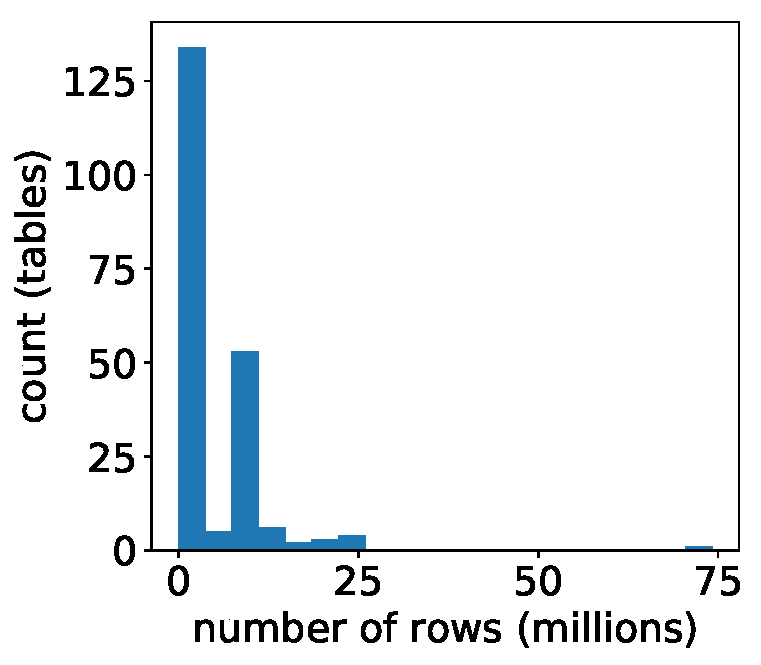
\includegraphics[width={1.0\linewidth}]{rows.pdf}
  \caption{Row distribution}
  \label{fig:pbib:generalstats:rows}
\end{subfigure}
% \hspace{1em}
\begin{subfigure}[t]{0.35\linewidth}
  \centering
  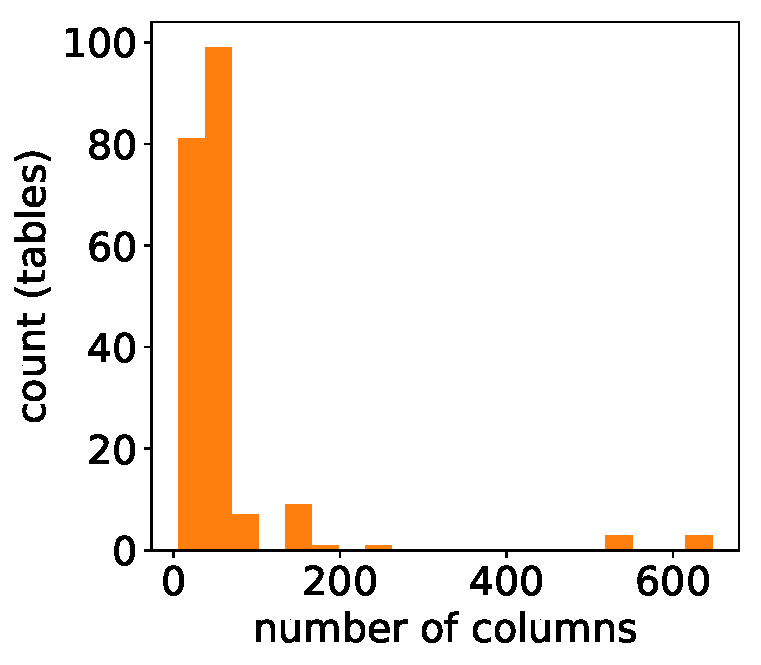
\includegraphics[width={1.0\linewidth}]{column_count.pdf}
  \caption{Column distribution}
  \label{fig:pbib:generalstats:columns}
\end{subfigure}
% \hspace{1em}
\begin{subfigure}[t]{0.35\linewidth}
  \centering
  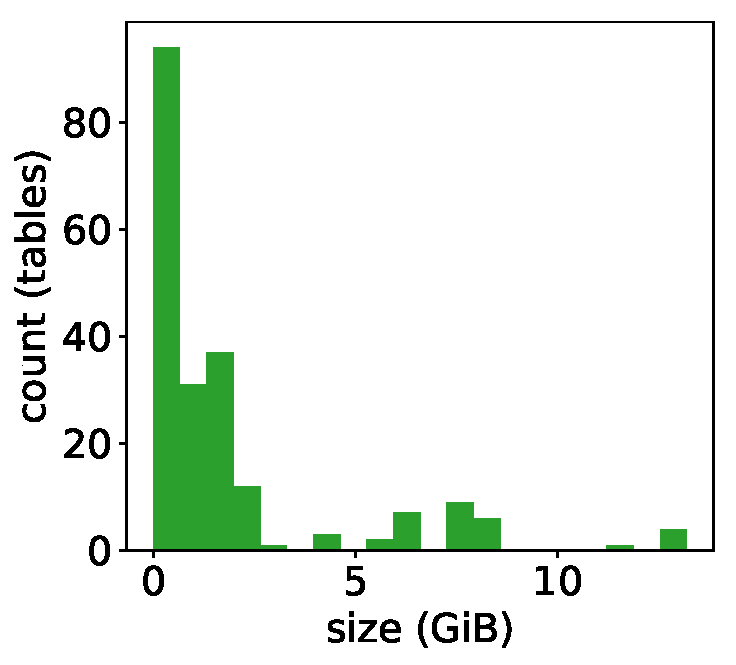
\includegraphics[width={1.0\linewidth}]{size_csv.pdf}
  \caption{Data size distribution}
  \label{fig:pbib:generalstats:size}
\end{subfigure}
}
\caption{Row, column and size distribution}
\label{fig:pbib:generalstats}
\end{figure}

\begin{figure}[h]
\centering
\makebox[\textwidth][c]{
\begin{subfigure}[t]{0.55\linewidth}
  \centering
  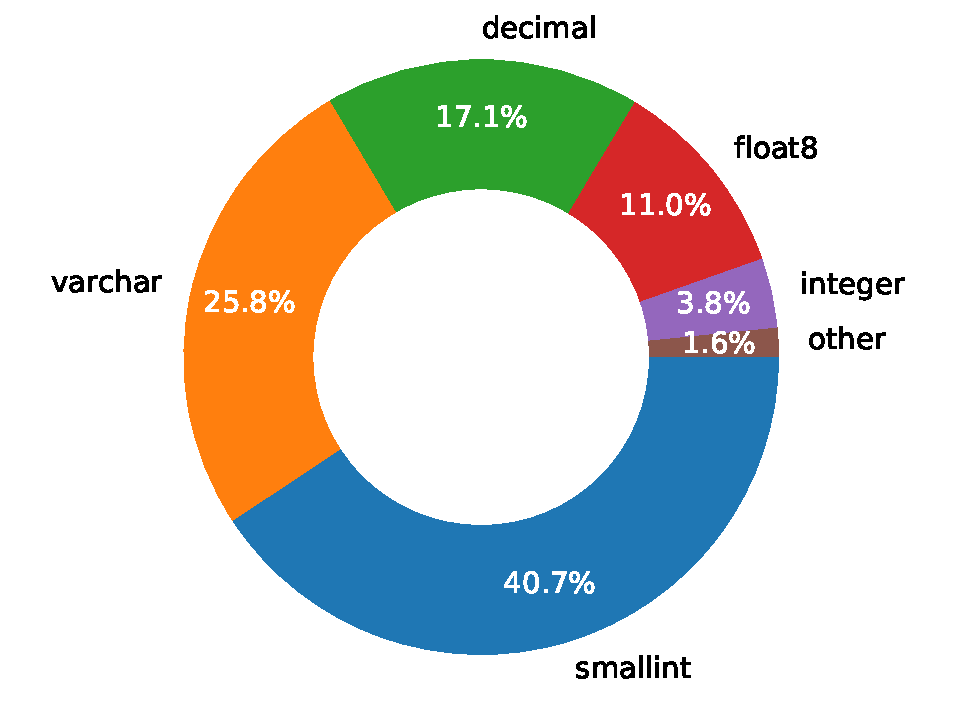
\includegraphics[width={1.0\linewidth}]{datatypes_total.pdf}
  \caption{Datatypes distribution}
  \label{fig:pbib:columnstats:datatypes}
\end{subfigure}
% \hspace{1em}
\begin{subfigure}[t]{0.55\linewidth}
  \centering
  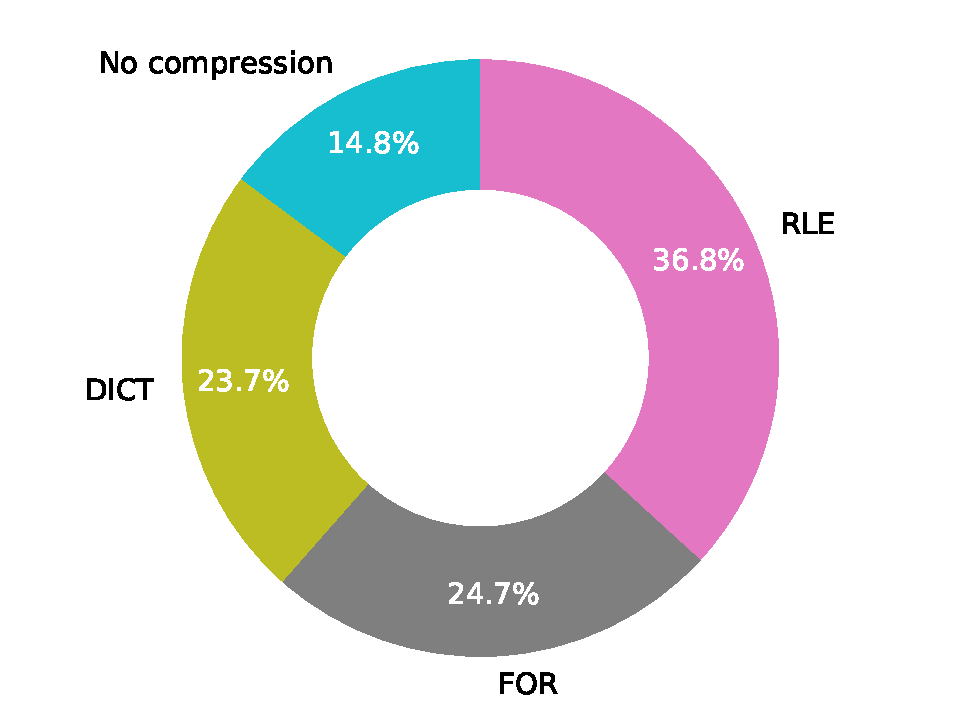
\includegraphics[width={1.0\linewidth}]{compression_methods_total.pdf}
  \caption{Compression potential}
  \label{fig:pbib:columnstats:estimators}
\end{subfigure}
}
\caption{Column statistics (percentage of columns)}
\label{fig:pbib:columnstats}
\end{figure}

Figure~\ref{fig:pbib:columnstats:datatypes} shows the distribution of datatypes across columns. The majority of the columns are numeric (73\%), followed by strings (25\%). The remaining columns are: \verb|DATE| (0.86\%), \verb|TIMESTAMP| (0.41\%), \verb|BIGINT| (0.17\%), \verb|BOOLEAN| (0.1\%), \verb|TIME| (0.05\%).

Given the focus of this thesis, we are interested in how suitable is the data for compression. We evaluated the potential of each column for compression with existing lightweight schemes: Run Length Encoding (RLE), Frame of Reference (FOR), Dictionary encoding (DICT). The evaluation was performed using the compression estimators defined in \ref{sub:estimators}~\nameref{sub:estimators}, following the methodology presented in \ref{fig:eval:methodology:estimatorbaseline}~\nameref{fig:eval:methodology:estimatorbaseline}. In short, we estimated the size of each column as compressed with RLE, FOR, DICT and uncompressed---based on a sample---and marked the column as a candidate for the method that gave the smallest size. The results are presented in Figure~\ref{fig:pbib:columnstats:estimators}. 85\% of the columns are good candidates for compression with lightweight schemes, while only 15\% of the columns are better left uncompressed. We applied DICT for \verb|VARCHAR| columns and RLE and FOR for \verb|numeric| columns. Most of the numeric columns are good candidates for RLE and FOR and the vast majority of \verb|VARCHAR| columns are dictionary compressible. The purpose of this analysis was to estimate the compression potential of the datasets in the benchmark. A more thorough analysis showing compression ratios and sizes is performed in \ref{sec:eval:resultsdiscussion}~\nameref{sec:eval:resultsdiscussion}.

\begin{figure}[h]
\centering
\makebox[\textwidth][c]{
\begin{subfigure}[t]{0.359\linewidth}
  \centering
  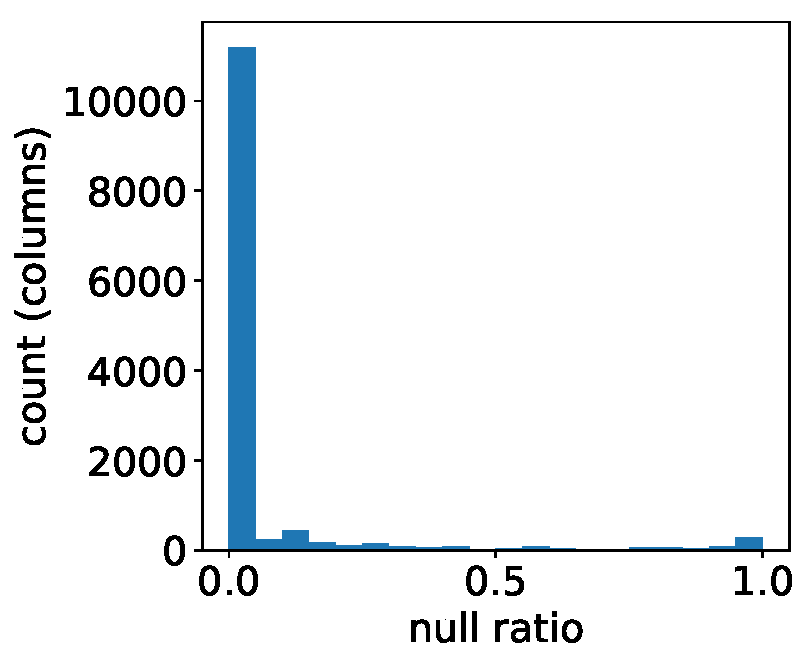
\includegraphics[width={1.0\linewidth}]{null_ratio.pdf}
  \caption{Null ratio}
  \label{fig:pbib:datastats:nulls}
\end{subfigure}
% \hspace{1em}
\begin{subfigure}[t]{0.35\linewidth}
  \centering
  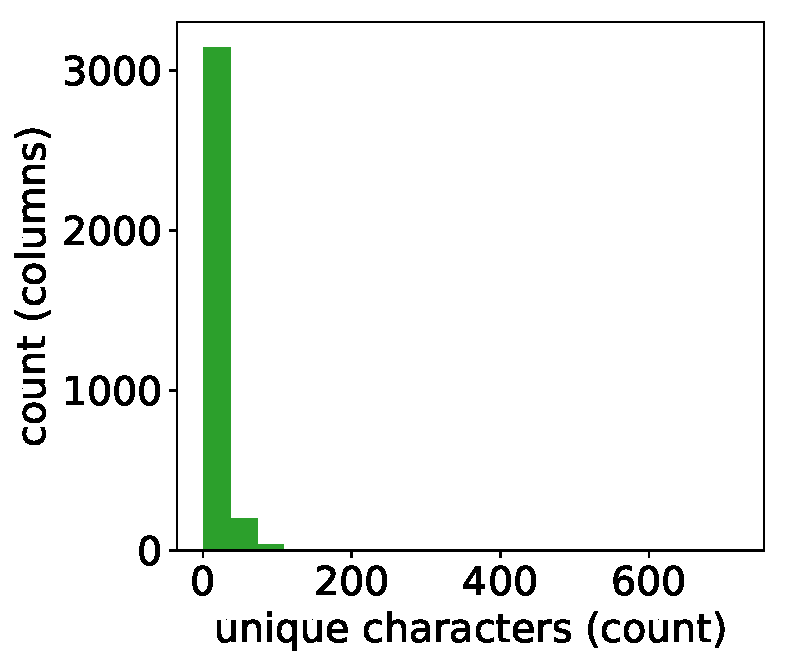
\includegraphics[width={1.0\linewidth}]{unique_chars.pdf}
  \caption{Unique characters}
  \label{fig:pbib:datastats:uniquechars}
\end{subfigure}
% \hspace{1em}
\begin{subfigure}[t]{0.359\linewidth}
  \centering
  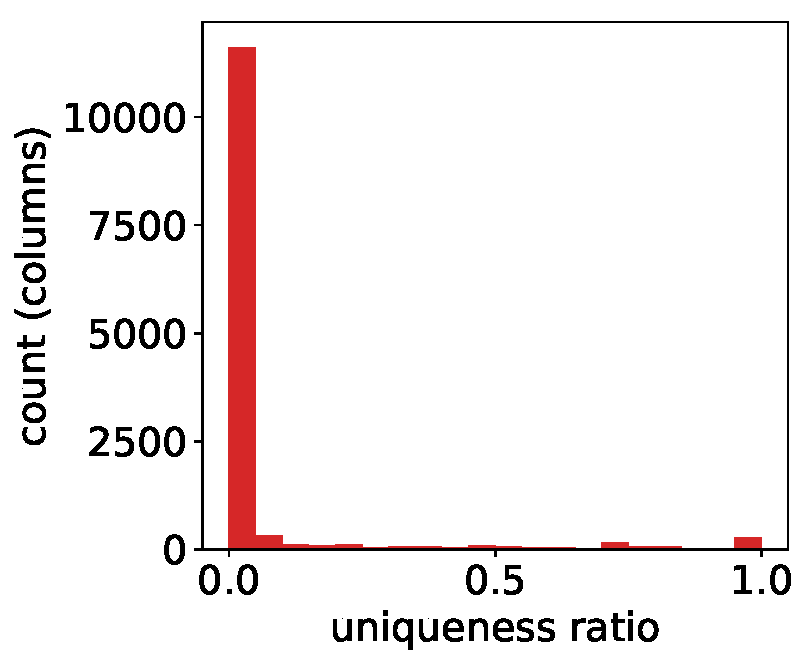
\includegraphics[width={1.0\linewidth}]{uniqueness_ratio.pdf}
  \caption{Uniqueness ratio}
  \label{fig:pbib:datastats:uniquenessratio}
\end{subfigure}
}
\caption{Data characterisation}
\label{fig:pbib:datastats}
\end{figure}

Figure~\ref{fig:pbib:datastats} shows metrics extracted with the \verb|statdump| command after loading the data into VectorWise \cite{zukowski2012vectorwise}. The percentage of null values is low for most of the columns. Figure~\ref{fig:pbib:datastats:uniquechars} shows the number of unique characters per column---for \verb|VARCHAR| columns: almost all of them have less than 100 unique characters. Only 8 columns have more than 255 unique characters and they contain social media content: posts or comments with hashtags and emoticons. Figure~\ref{fig:pbib:datastats:uniquenessratio} shows the uniqueness ratio of all the columns, irrespective of their datatype. The uniqueness of a column is computed as the number of unique values divided by the total number of values: \(\frac{unique_{count}}{total_{count}}\). Note that these metrics were computed based on the entire data and not based on a sample, therefore they are accurate. We notice how almost all of the columns have a very low uniqueness, indicating a high degree of repetition. This property makes the data suitable for compression and confirms the compression estimation results.
% \newline
% \newline

\subsection{Manual analysis}
So far we showed a general characterisation of the benchmark, mostly from a statistical point of view. In order to better understand the properties of real data and to gain more insight about it, we manually searched for patterns---common ways that users represent the data---with the purpose of finding opportunities for more compact representations. Below is a list of our findings:

\begin{itemize}
    % \item unstructured text
    % \item social media content---e.g. usernames, personal \& contact details, posts, comments, hashtags, emoticons
    % \item extended character set---UTF-8 characters from different languages, emoticons, etc.

    \item empty/missing values that are not nulls---e.g. empty quotes, whitespace characters;\\ examples:
    Eixo\_1\footnotemark: comunidade\_quilombola, unidade\_demandante
    
    \footnotetext{\url{https://github.com/cwida/public_bi_benchmark/blob/master/benchmark/Eixo/samples/Eixo\_1.sample.csv}}
    
    \item leading/trailing whitespace, some with the purpose of ensuring a common length of the values on \verb|VARCHAR| columns;\\ examples:
    CommonGovernment\_1\footnotemark: contract\_num, primary\_contract\_piid
    
    \item numbers and dates stored as strings in \verb|VARCHAR| columns;\\ examples:
    CommonGovernment\_1\footnotemark[\value{footnote}]: contract\_signeddate, agency\_code
    
    \item strings with fixed structure composed of substrings from different distributions---e.g. emails, urls, strings starting with a constant and ending in a number;\\ examples:
    CommonGovernment\_1\footnotemark[\value{footnote}]: co\_name, contract\_num
    
    \item correlations between columns---mostly as categorical variables, but also numeric correlations; special cases: identical columns;\\ examples:
    CommonGovernment\_1\footnotemark[\value{footnote}]: short\_name, ag\_name, description
    
    \footnotetext{\url{https://github.com/cwida/public_bi_benchmark/blob/master/benchmark/CommonGovernment/samples/CommonGovernment_1.sample.csv}}
\end{itemize}

All of these patterns are inefficient representations of the information, in terms of data storage. Some of them could have been avoided by the user (e.g. choosing the proper datatype for numeric values), while others are determined by the nature of the data itself. These patterns represent compression opportunities that cannot be exploited through existing compression schemes.
% \newline
% \newline
\subsection{Conclusion}
The conclusion that we can draw from the analysis we performed on the Public BI benchmark is that real data is redundant and represented in inefficient ways. It is already suitable for compression with existing lightweight methods, but it has a considerable untapped compression potential that could be exploited if the data had a different representation.

\iffalse
- scatter plot with skewness and kurtosis on distribution types background (see link from Benno) (Min/Max; Outliers characterisation; standard deviation; check if normal distribution; (in terms of distribution of numbers, dates, length of strings, character sets used, etc); metrics: range & standard deviation, mean (big skew = large range & big stdev), measures of spread = range and stdev)
\fi

% ---------------------------------------------------------------------------
% ----------------------- end of thesis sub-document ------------------------
% ---------------------------------------------------------------------------